\documentclass[tikz,border=9pt]{standalone}
\usepackage[T1]{fontenc}
\usepackage{lmodern,amsmath}
\usetikzlibrary{arrows.meta}
\definecolor{ink}{HTML}{183444}
\definecolor{blue}{HTML}{1B6780}
\definecolor{amber}{HTML}{AD601A}
\begin{document}
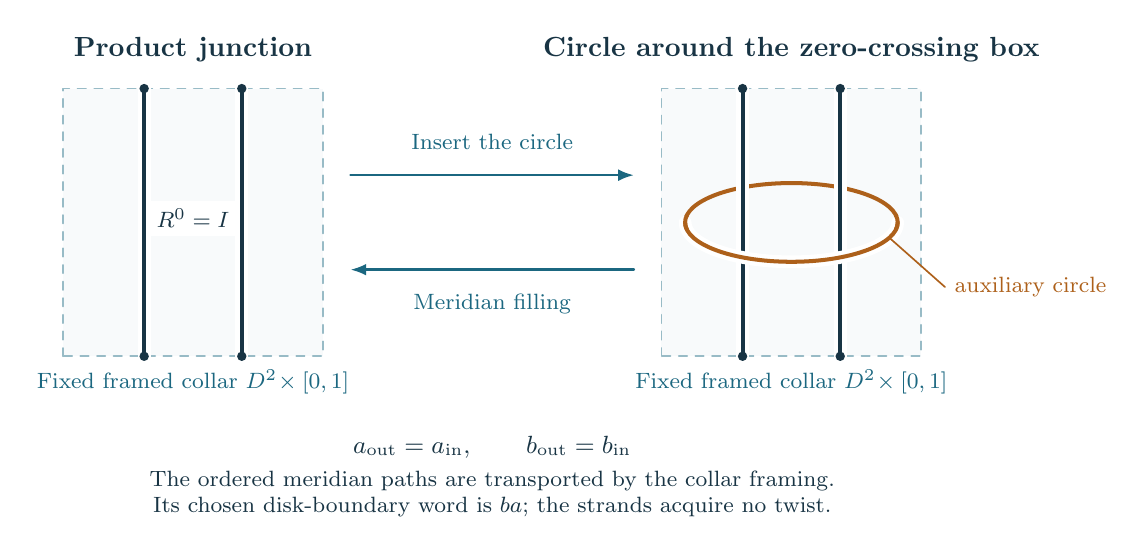
\begin{tikzpicture}[x=1cm,y=1cm,font=\small,text=ink,
  line cap=round,line join=round,
  strand/.style={draw=ink,line width=1.5pt,
    preaction={draw=white,line width=4.6pt}},
  circlearc/.style={draw=amber,line width=1.45pt},
  move/.style={-{Latex[length=2mm]},draw=blue,line width=.9pt}]
% The collar framing and the two endpoint positions are identical in both panels.
\foreach \cx in {-3.8,3.8}{
  \begin{scope}[shift={(\cx,0)}]
    \fill[blue!3] (-1.65,-1.7) rectangle (1.65,1.7);
    \draw[blue!45,dashed,line width=.65pt]
       (-1.65,-1.7) rectangle (1.65,1.7);
    \node[font=\footnotesize,text=blue] at (0,-2.03)
      {Fixed framed collar $D^2\!\times[0,1]$};
  \end{scope}
}
\begin{scope}[shift={(-3.8,0)}]
  \node[font=\bfseries] at (0,2.2) {Product junction};
  \foreach \xx in {-.62,.62}{
    \draw[strand] (\xx,-1.7)--(\xx,1.7);
    \fill[ink] (\xx,-1.7) circle (1.7pt);
    \fill[ink] (\xx,1.7) circle (1.7pt);
  }
  \node[fill=white,inner sep=3pt,font=\footnotesize] at (0,.05)
    {$R^0=I$};
\end{scope}
\begin{scope}[shift={(3.8,0)}]
  \node[font=\bfseries] at (0,2.2) {Circle around the zero-crossing box};
  % Back semicircle lies behind both strands. Their white underlay cuts it.
  \draw[circlearc] (1.35,0)
    arc[start angle=0,end angle=180,x radius=1.35cm,y radius=.50cm];
  \foreach \xx in {-.62,.62}{
    \draw[strand] (\xx,-1.7)--(\xx,1.7);
    \fill[ink] (\xx,-1.7) circle (1.7pt);
    \fill[ink] (\xx,1.7) circle (1.7pt);
  }
  % Front semicircle crosses over both strands, with a visible gap underneath.
  \draw[circlearc,preaction={draw=white,line width=4.6pt}]
    (-1.35,0) arc[start angle=180,end angle=360,
      x radius=1.35cm,y radius=.50cm];
  % Restore the two side joins after the front arc's crossing underlay.
  \draw[circlearc] ({1.35*cos(170)},{.50*sin(170)})
    arc[start angle=170,end angle=190,x radius=1.35cm,y radius=.50cm];
  \draw[circlearc] ({1.35*cos(350)},{.50*sin(350)})
    arc[start angle=350,end angle=370,x radius=1.35cm,y radius=.50cm];
  \draw[amber,line width=.6pt] (1.25,-.20)--(1.95,-.82);
  \node[anchor=west,text=amber,font=\footnotesize] at (1.95,-.82)
    {auxiliary circle};
\end{scope}
\draw[move] (-1.8,.6)--(1.8,.6);
\node[align=center,font=\footnotesize,text=blue] at (0,1.03)
  {Insert the circle};
\draw[move] (1.8,-.6)--(-1.8,-.6);
\node[align=center,font=\footnotesize,text=blue] at (0,-1.03)
  {Meridian filling};
\node[align=center] at (0,-2.85)
  {$a_{\mathrm{out}}=a_{\mathrm{in}},\qquad
    b_{\mathrm{out}}=b_{\mathrm{in}}$};
\node[align=center,font=\footnotesize,text width=11.2cm] at (0,-3.45)
  {The ordered meridian paths are transported by the collar framing.
   Its chosen disk-boundary word is $ba$; the strands acquire no twist.};
\end{tikzpicture}
\end{document}
